\documentclass[tikz,border=10pt]{standalone}
\usepackage[T1]{fontenc}
\usepackage{helvet}
\renewcommand{\familydefault}{\sfdefault}
\usepackage{amsmath,amssymb}
\usepackage{tikz}
\usetikzlibrary{calc,positioning,fit,arrows.meta,shapes.geometric}

% Canonical Academic Palette
\definecolor{OxfordNavy}{HTML}{1E293B}
\definecolor{SlateSteel}{HTML}{334155}
\definecolor{MutedTeal}{HTML}{0F766E}
\definecolor{TealL0}{HTML}{F0FDFA}
\definecolor{Burgundy}{HTML}{991B1B}
\definecolor{BurgundyL0}{HTML}{FEF2F2}
\definecolor{WarmOchre}{HTML}{92400E}
\definecolor{OchreL0}{HTML}{FFFBEB}
\definecolor{ForestSage}{HTML}{166534}
\definecolor{SageL0}{HTML}{F0FDF4}
\definecolor{CoolParchment}{HTML}{F8FAFC}
\definecolor{SlateRim}{HTML}{CBD5E1}
\definecolor{GoldPin}{HTML}{D97706}
\definecolor{DarkSlate}{HTML}{0F172A}

\begin{document}
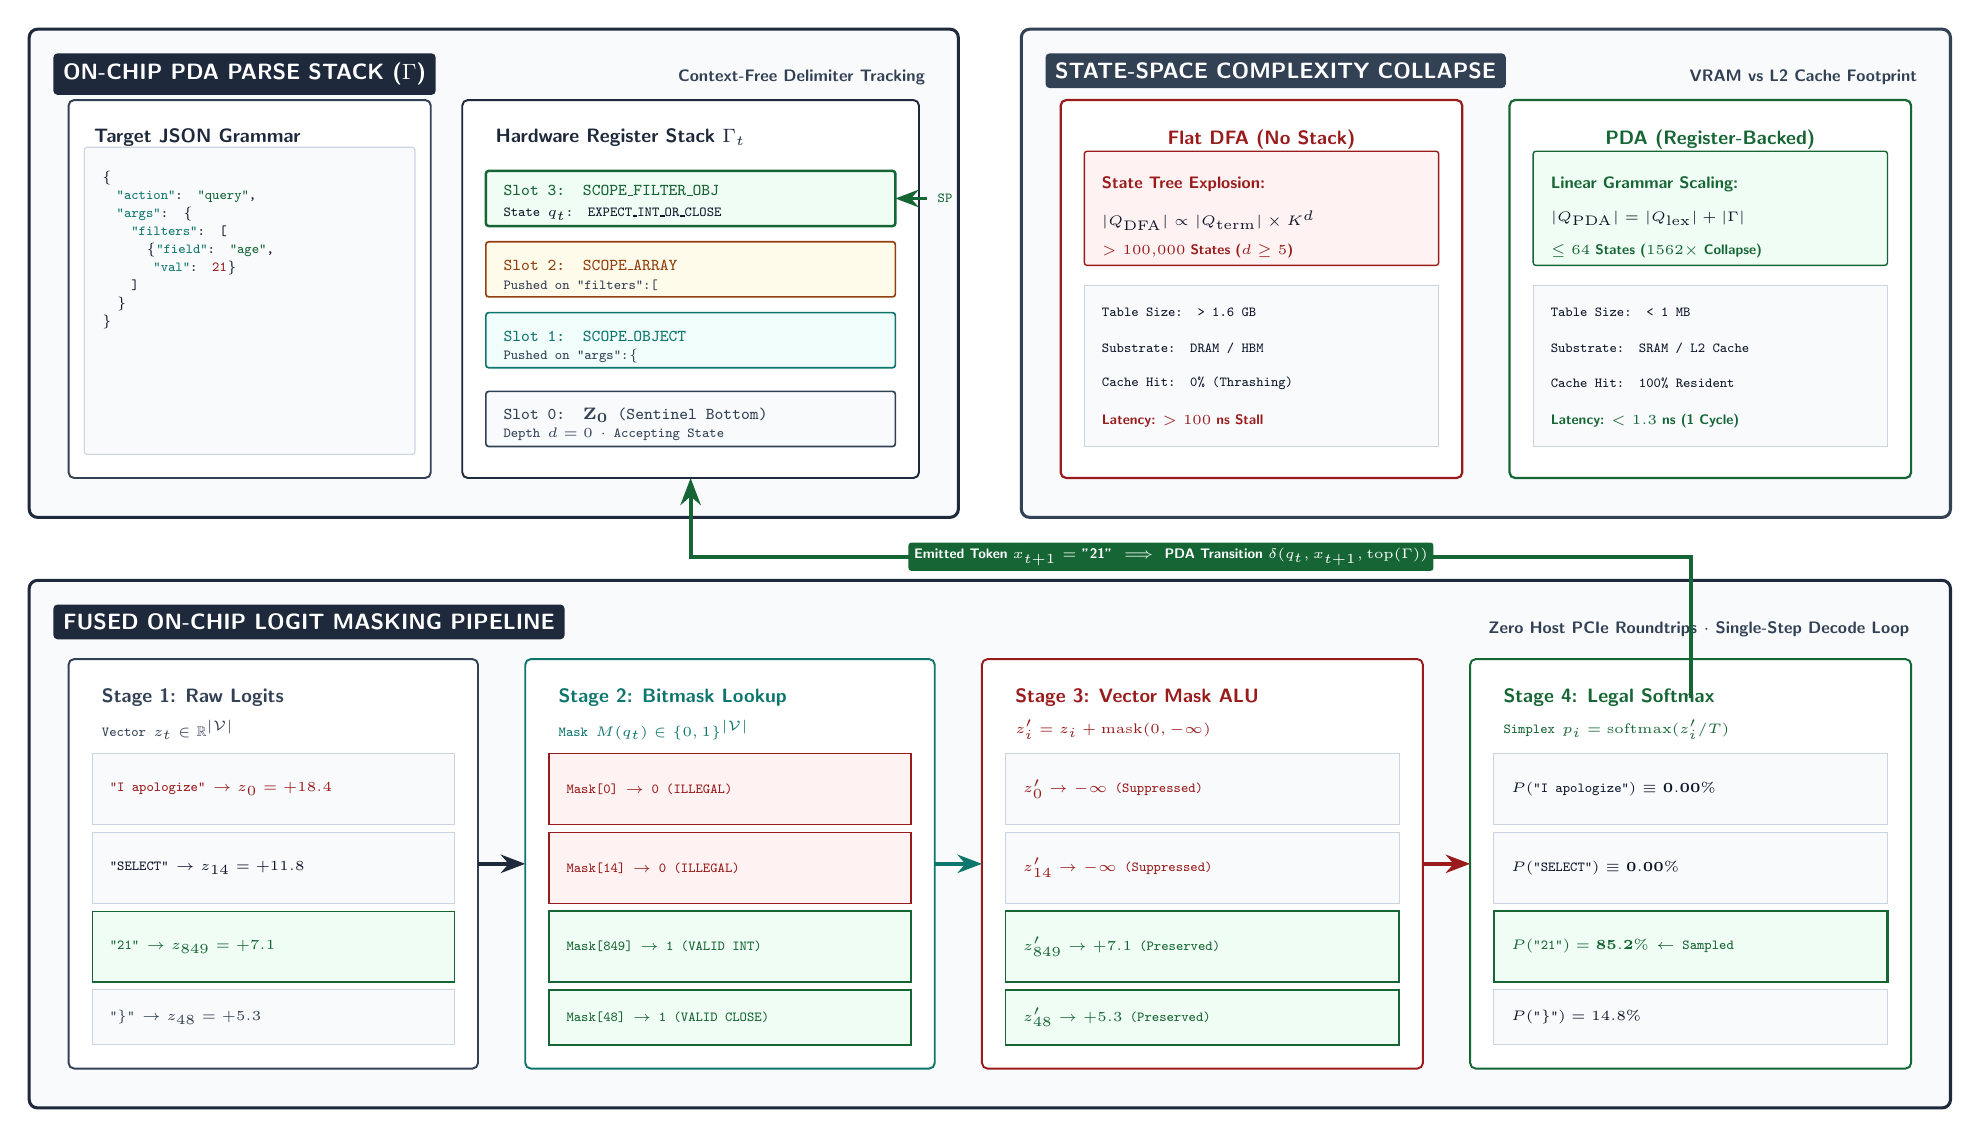
\begin{tikzpicture}[
  font=\sffamily,
  scale=1.0,
  >=Stealth,
  node distance=0.5cm
]

% =============================================================================
% TOP TIER: RECURSIVE SCHEMA & HARDWARE PARSE STACK (Gamma)
% =============================================================================

% Left Unit: Formal Recursive Grammar & Stack Lifecycle
\begin{scope}[shift={(0, 7.8)}]
  \draw[fill=CoolParchment, draw=OxfordNavy, line width=1.1pt, rounded corners=3pt]
    (0, 0) rectangle (11.8, 6.2);

  \node[anchor=north west, fill=OxfordNavy, text=white, font=\fontsize{8.5}{10}\selectfont\bfseries, rounded corners=1.5pt, inner sep=3.5pt]
    at (0.3, 5.9) {ON-CHIP PDA PARSE STACK ($\Gamma$)};
  \node[anchor=north east, text=SlateSteel, font=\fontsize{6.5}{8}\selectfont\bfseries]
    at (11.5, 5.8) {Context-Free Delimiter Tracking};

  % Unit 1A: Target Schema Code Segment
  \begin{scope}[shift={(0.5, 0.5)}]
    \draw[fill=white, draw=SlateSteel, line width=0.7pt, rounded corners=2pt] (0, 0) rectangle (4.6, 4.8);
    \node[anchor=north west, text=OxfordNavy, font=\fontsize{7.2}{8.5}\selectfont\bfseries] at (0.2, 4.55) {Target JSON Grammar};
    
    % Monospace AST Schema
    \draw[fill=CoolParchment, draw=SlateRim, rounded corners=1pt] (0.2, 0.3) rectangle (4.4, 4.2);
    \node[anchor=north west, font=\fontsize{5.2}{6.5}\selectfont\ttfamily, text=DarkSlate] at (0.3, 4.05) {
      \begin{tabular}{@{}l@{}}
        \{\\
        \ \ \textcolor{MutedTeal}{"action"}: \textcolor{ForestSage}{"query"},\\
        \ \ \textcolor{MutedTeal}{"args"}: \{\\
        \ \ \ \ \textcolor{MutedTeal}{"filters"}: [\\
        \ \ \ \ \ \ \{\textcolor{MutedTeal}{"field"}: \textcolor{ForestSage}{"age"},\\
        \ \ \ \ \ \ \ \textcolor{MutedTeal}{"val"}: \textcolor{Burgundy}{\textbf{21}}\}\\
        \ \ \ \ ]\\
        \ \ \}\\
        \}
      \end{tabular}
    };
  \end{scope}

  % Unit 1B: Hardware Pushdown Register Stack (Vertical Register File)
  \begin{scope}[shift={(5.5, 0.5)}]
    \draw[fill=white, draw=OxfordNavy, line width=0.7pt, rounded corners=2pt] (0, 0) rectangle (5.8, 4.8);
    \node[anchor=north west, text=OxfordNavy, font=\fontsize{7.2}{8.5}\selectfont\bfseries] at (0.3, 4.55) {Hardware Register Stack $\Gamma_t$};

    % Stack slots
    % Slot 3 (Active Top)
    \draw[fill=SageL0, draw=ForestSage, line width=0.9pt, rounded corners=1pt] (0.3, 3.2) rectangle (5.5, 3.9);
    \node[anchor=west, font=\fontsize{5.8}{7}\selectfont\ttfamily\bfseries, text=ForestSage] at (0.4, 3.65) {Slot 3: SCOPE\_FILTER\_OBJ};
    \node[anchor=west, font=\fontsize{5.0}{6}\selectfont\ttfamily, text=DarkSlate] at (0.4, 3.35) {State $q_t$: \textbf{EXPECT\_INT\_OR\_CLOSE}};
    % Stack pointer arrow
    \draw[<-, draw=ForestSage, line width=1.2pt] (5.5, 3.55) -- (5.9, 3.55)
      node[right, font=\fontsize{5.5}{6.5}\selectfont\bfseries\ttfamily, text=ForestSage] {SP};

    % Slot 2
    \draw[fill=OchreL0, draw=WarmOchre, line width=0.6pt, rounded corners=1pt] (0.3, 2.3) rectangle (5.5, 3.0);
    \node[anchor=west, font=\fontsize{5.8}{7}\selectfont\ttfamily, text=WarmOchre] at (0.4, 2.7) {Slot 2: SCOPE\_ARRAY};
    \node[anchor=west, font=\fontsize{5.0}{6}\selectfont\ttfamily, text=SlateSteel] at (0.4, 2.45) {Pushed on \texttt{"filters":[}};

    % Slot 1
    \draw[fill=TealL0, draw=MutedTeal, line width=0.6pt, rounded corners=1pt] (0.3, 1.4) rectangle (5.5, 2.1);
    \node[anchor=west, font=\fontsize{5.8}{7}\selectfont\ttfamily, text=MutedTeal] at (0.4, 1.8) {Slot 1: SCOPE\_OBJECT};
    \node[anchor=west, font=\fontsize{5.0}{6}\selectfont\ttfamily, text=SlateSteel] at (0.4, 1.55) {Pushed on \texttt{"args":\{}};

    % Slot 0 (Bottom Sentinel)
    \draw[fill=CoolParchment, draw=SlateSteel, line width=0.6pt, rounded corners=1pt] (0.3, 0.4) rectangle (5.5, 1.1);
    \node[anchor=west, font=\fontsize{5.8}{7}\selectfont\ttfamily\bfseries, text=SlateSteel] at (0.4, 0.8) {Slot 0: $\mathbf{Z_0}$ (Sentinel Bottom)};
    \node[anchor=west, font=\fontsize{5.0}{6}\selectfont\ttfamily, text=SlateSteel] at (0.4, 0.55) {Depth $d = 0$ $\cdot$ Accepting State};
  \end{scope}

\end{scope}


% Right Unit: The State Space Collapse (Flat DFA vs PDA)
\begin{scope}[shift={(12.6, 7.8)}]
  \draw[fill=CoolParchment, draw=SlateSteel, line width=1.1pt, rounded corners=3pt]
    (0, 0) rectangle (11.8, 6.2);

  \node[anchor=north west, fill=SlateSteel, text=white, font=\fontsize{8.5}{10}\selectfont\bfseries, rounded corners=1.5pt, inner sep=3.5pt]
    at (0.3, 5.9) {STATE-SPACE COMPLEXITY COLLAPSE};
  \node[anchor=north east, text=SlateSteel, font=\fontsize{6.5}{8}\selectfont\bfseries]
    at (11.5, 5.8) {VRAM vs L2 Cache Footprint};

  % Sub-box Left: Flat DFA State Explosion
  \begin{scope}[shift={(0.5, 0.5)}]
    \draw[fill=white, draw=Burgundy, line width=0.8pt, rounded corners=2pt] (0, 0) rectangle (5.1, 4.8);
    \node[anchor=north, text=Burgundy, font=\fontsize{7.2}{8.5}\selectfont\bfseries] at (2.55, 4.55) {Flat DFA (No Stack)};

    % Metrics card
    \draw[fill=BurgundyL0, draw=Burgundy, line width=0.5pt, rounded corners=1pt] (0.3, 2.7) rectangle (4.8, 4.15);
    \node[anchor=north west, text=Burgundy, font=\fontsize{6.0}{7}\selectfont\bfseries] at (0.4, 3.95) {State Tree Explosion:};
    \node[anchor=north west, text=DarkSlate, font=\fontsize{5.2}{6.2}\selectfont\ttfamily] at (0.4, 3.52) {$|Q_{\mathrm{DFA}}| \propto |Q_{\mathrm{term}}| \times K^d$};
    \node[anchor=north west, text=Burgundy, font=\fontsize{5.2}{6.2}\selectfont\bfseries] at (0.4, 3.10) {$> 100{,}000$ States ($d \ge 5$)};

    % Footprint & Bottleneck
    \draw[fill=CoolParchment, draw=SlateRim] (0.3, 0.4) rectangle (4.8, 2.45);
    \node[anchor=west, text=DarkSlate, font=\fontsize{5.2}{6.2}\selectfont\ttfamily] at (0.4, 2.1) {Table Size: \textbf{> 1.6 GB}};
    \node[anchor=west, text=DarkSlate, font=\fontsize{5.2}{6.2}\selectfont\ttfamily] at (0.4, 1.65) {Substrate: \textbf{DRAM / HBM}};
    \node[anchor=west, text=DarkSlate, font=\fontsize{5.2}{6.2}\selectfont\ttfamily] at (0.4, 1.2) {Cache Hit: \textbf{0\% (Thrashing)}};
    \node[anchor=west, text=Burgundy, font=\fontsize{5.2}{6.2}\selectfont\bfseries] at (0.4, 0.72) {Latency: $> 100\text{ ns}$ Stall};
  \end{scope}

  % Sub-box Right: Pushdown Automaton
  \begin{scope}[shift={(6.2, 0.5)}]
    \draw[fill=white, draw=ForestSage, line width=0.8pt, rounded corners=2pt] (0, 0) rectangle (5.1, 4.8);
    \node[anchor=north, text=ForestSage, font=\fontsize{7.2}{8.5}\selectfont\bfseries] at (2.55, 4.55) {PDA (Register-Backed)};

    % Metrics card
    \draw[fill=SageL0, draw=ForestSage, line width=0.5pt, rounded corners=1pt] (0.3, 2.7) rectangle (4.8, 4.15);
    \node[anchor=north west, text=ForestSage, font=\fontsize{6.0}{7}\selectfont\bfseries] at (0.4, 3.95) {Linear Grammar Scaling:};
    \node[anchor=north west, text=DarkSlate, font=\fontsize{5.2}{6.2}\selectfont\ttfamily] at (0.4, 3.52) {$|Q_{\mathrm{PDA}}| = |Q_{\mathrm{lex}}| + |\Gamma|$};
    \node[anchor=north west, text=ForestSage, font=\fontsize{5.2}{6.2}\selectfont\bfseries] at (0.4, 3.10) {$\le 64$ States ($1562\times$ Collapse)};

    % Footprint & Advantage
    \draw[fill=CoolParchment, draw=SlateRim] (0.3, 0.4) rectangle (4.8, 2.45);
    \node[anchor=west, text=DarkSlate, font=\fontsize{5.2}{6.2}\selectfont\ttfamily] at (0.4, 2.1) {Table Size: \textbf{< 1 MB}};
    \node[anchor=west, text=DarkSlate, font=\fontsize{5.2}{6.2}\selectfont\ttfamily] at (0.4, 1.65) {Substrate: \textbf{SRAM / L2 Cache}};
    \node[anchor=west, text=DarkSlate, font=\fontsize{5.2}{6.2}\selectfont\ttfamily] at (0.4, 1.2) {Cache Hit: \textbf{100\% Resident}};
    \node[anchor=west, text=ForestSage, font=\fontsize{5.2}{6.2}\selectfont\bfseries] at (0.4, 0.72) {Latency: $< 1.3\text{ ns}$ (1 Cycle)};
  \end{scope}

\end{scope}


% =============================================================================
% BOTTOM TIER: 4-STAGE HARDWARE MASKING PIPELINE
% =============================================================================
\begin{scope}[shift={(0, 0.3)}]
  \draw[fill=CoolParchment, draw=OxfordNavy, line width=1.1pt, rounded corners=3pt]
    (0, 0) rectangle (24.4, 6.7);

  \node[anchor=north west, fill=OxfordNavy, text=white, font=\fontsize{8.5}{10}\selectfont\bfseries, rounded corners=1.5pt, inner sep=3.5pt]
    at (0.3, 6.4) {FUSED ON-CHIP LOGIT MASKING PIPELINE};
  \node[anchor=north east, text=SlateSteel, font=\fontsize{6.5}{8}\selectfont\bfseries]
    at (24.0, 6.3) {Zero Host PCIe Roundtrips $\cdot$ Single-Step Decode Loop};

  % Stage 1: Raw Unconstrained Logits
  \begin{scope}[shift={(0.5, 0.5)}]
    \draw[fill=white, draw=SlateSteel, line width=0.7pt, rounded corners=2pt] (0, 0) rectangle (5.2, 5.2);
    \node[anchor=north west, text=SlateSteel, font=\fontsize{6.8}{8}\selectfont\bfseries] at (0.3, 4.95) {Stage 1: Raw Logits};
    \node[anchor=north west, text=SlateSteel, font=\fontsize{5.0}{6}\selectfont\ttfamily] at (0.3, 4.55) {Vector $z_t \in \mathbb{R}^{|\mathcal{V}|}$};

    % Logit vector slots
    \draw[fill=CoolParchment, draw=SlateRim] (0.3, 3.1) rectangle (4.9, 4.0);
    \node[anchor=west, font=\fontsize{4.8}{5.8}\selectfont\ttfamily, text=Burgundy] at (0.4, 3.55) {"I apologize" $\to z_0 = +18.4$};

    \draw[fill=CoolParchment, draw=SlateRim] (0.3, 2.1) rectangle (4.9, 3.0);
    \node[anchor=west, font=\fontsize{4.8}{5.8}\selectfont\ttfamily, text=DarkSlate] at (0.4, 2.55) {"SELECT" $\to z_{14} = +11.8$};

    \draw[fill=SageL0, draw=ForestSage] (0.3, 1.1) rectangle (4.9, 2.0);
    \node[anchor=west, font=\fontsize{4.8}{5.8}\selectfont\ttfamily\bfseries, text=ForestSage] at (0.4, 1.55) {"21" $\to z_{849} = +7.1$};

    \draw[fill=CoolParchment, draw=SlateRim] (0.3, 0.3) rectangle (4.9, 1.0);
    \node[anchor=west, font=\fontsize{4.8}{5.8}\selectfont\ttfamily, text=SlateSteel] at (0.4, 0.65) {"\}" $\to z_{48} = +5.3$};
  \end{scope}

  % Arrow S1 -> S2
  \draw[->, line width=1.3pt, draw=OxfordNavy] (5.7, 3.1) -- (6.3, 3.1);

  % Stage 2: L2 Cache Bitmask Lookup
  \begin{scope}[shift={(6.3, 0.5)}]
    \draw[fill=white, draw=MutedTeal, line width=0.7pt, rounded corners=2pt] (0, 0) rectangle (5.2, 5.2);
    \node[anchor=north west, text=MutedTeal, font=\fontsize{6.8}{8}\selectfont\bfseries] at (0.3, 4.95) {Stage 2: Bitmask Lookup};
    \node[anchor=north west, text=MutedTeal, font=\fontsize{5.0}{6}\selectfont\ttfamily] at (0.3, 4.55) {Mask $M(q_t) \in \{0, 1\}^{|\mathcal{V}|}$};

    % Bitmask cells
    \draw[fill=BurgundyL0, draw=Burgundy, line width=0.5pt] (0.3, 3.1) rectangle (4.9, 4.0);
    \node[anchor=west, font=\fontsize{4.8}{5.8}\selectfont\ttfamily\bfseries, text=Burgundy] at (0.4, 3.55) {Mask[0] $\to$ 0 (ILLEGAL)};

    \draw[fill=BurgundyL0, draw=Burgundy, line width=0.5pt] (0.3, 2.1) rectangle (4.9, 3.0);
    \node[anchor=west, font=\fontsize{4.8}{5.8}\selectfont\ttfamily\bfseries, text=Burgundy] at (0.4, 2.55) {Mask[14] $\to$ 0 (ILLEGAL)};

    \draw[fill=SageL0, draw=ForestSage, line width=0.7pt] (0.3, 1.1) rectangle (4.9, 2.0);
    \node[anchor=west, font=\fontsize{4.8}{5.8}\selectfont\ttfamily\bfseries, text=ForestSage] at (0.4, 1.55) {Mask[849] $\to$ 1 (VALID INT)};

    \draw[fill=SageL0, draw=ForestSage, line width=0.7pt] (0.3, 0.3) rectangle (4.9, 1.0);
    \node[anchor=west, font=\fontsize{4.8}{5.8}\selectfont\ttfamily\bfseries, text=ForestSage] at (0.4, 0.65) {Mask[48] $\to$ 1 (VALID CLOSE)};
  \end{scope}

  % Arrow S2 -> S3
  \draw[->, line width=1.3pt, draw=MutedTeal] (11.5, 3.1) -- (12.1, 3.1);

  % Stage 3: Vectorized Slicing ALU
  \begin{scope}[shift={(12.1, 0.5)}]
    \draw[fill=white, draw=Burgundy, line width=0.7pt, rounded corners=2pt] (0, 0) rectangle (5.6, 5.2);
    \node[anchor=north west, text=Burgundy, font=\fontsize{6.8}{8}\selectfont\bfseries] at (0.3, 4.95) {Stage 3: Vector Mask ALU};
    \node[anchor=north west, text=Burgundy, font=\fontsize{5.0}{6}\selectfont\ttfamily] at (0.3, 4.55) {$z'_i = z_i + \mathrm{mask}(0, -\infty)$};

    % Clamped values
    \draw[fill=CoolParchment, draw=SlateRim] (0.3, 3.1) rectangle (5.3, 4.0);
    \node[anchor=west, font=\fontsize{4.8}{5.8}\selectfont\ttfamily, text=Burgundy] at (0.4, 3.55) {$z'_0 \to -\infty$ \textbf{(Suppressed)}};

    \draw[fill=CoolParchment, draw=SlateRim] (0.3, 2.1) rectangle (5.3, 3.0);
    \node[anchor=west, font=\fontsize{4.8}{5.8}\selectfont\ttfamily, text=Burgundy] at (0.4, 2.55) {$z'_{14} \to -\infty$ \textbf{(Suppressed)}};

    \draw[fill=SageL0, draw=ForestSage, line width=0.6pt] (0.3, 1.1) rectangle (5.3, 2.0);
    \node[anchor=west, font=\fontsize{4.8}{5.8}\selectfont\ttfamily\bfseries, text=ForestSage] at (0.4, 1.55) {$z'_{849} \to +7.1$ \textbf{(Preserved)}};

    \draw[fill=SageL0, draw=ForestSage, line width=0.6pt] (0.3, 0.3) rectangle (5.3, 1.0);
    \node[anchor=west, font=\fontsize{4.8}{5.8}\selectfont\ttfamily\bfseries, text=ForestSage] at (0.4, 0.65) {$z'_{48} \to +5.3$ \textbf{(Preserved)}};
  \end{scope}

  % Arrow S3 -> S4
  \draw[->, line width=1.3pt, draw=Burgundy] (17.7, 3.1) -- (18.3, 3.1);

  % Stage 4: Softmax Simplex Sampler
  \begin{scope}[shift={(18.3, 0.5)}]
    \draw[fill=white, draw=ForestSage, line width=0.7pt, rounded corners=2pt] (0, 0) rectangle (5.6, 5.2);
    \node[anchor=north west, text=ForestSage, font=\fontsize{6.8}{8}\selectfont\bfseries] at (0.3, 4.95) {Stage 4: Legal Softmax};
    \node[anchor=north west, text=ForestSage, font=\fontsize{5.0}{6}\selectfont\ttfamily] at (0.3, 4.55) {Simplex $p_i = \mathrm{softmax}(z'_i / T)$};

    % Probabilities
    \draw[fill=CoolParchment, draw=SlateRim] (0.3, 3.1) rectangle (5.3, 4.0);
    \node[anchor=west, font=\fontsize{4.8}{5.8}\selectfont\ttfamily, text=DarkSlate] at (0.4, 3.55) {$P(\text{"I apologize"}) \equiv \mathbf{0.00\%}$};

    \draw[fill=CoolParchment, draw=SlateRim] (0.3, 2.1) rectangle (5.3, 3.0);
    \node[anchor=west, font=\fontsize{4.8}{5.8}\selectfont\ttfamily, text=DarkSlate] at (0.4, 2.55) {$P(\text{"SELECT"}) \equiv \mathbf{0.00\%}$};

    \draw[fill=SageL0, draw=ForestSage, line width=0.8pt] (0.3, 1.1) rectangle (5.3, 2.0);
    \node[anchor=west, font=\fontsize{4.8}{5.8}\selectfont\ttfamily\bfseries, text=ForestSage] at (0.4, 1.55) {$P(\text{"21"}) = \mathbf{85.2\%}$ $\leftarrow$ \textbf{Sampled}};

    \draw[fill=CoolParchment, draw=SlateRim] (0.3, 0.3) rectangle (5.3, 1.0);
    \node[anchor=west, font=\fontsize{4.8}{5.8}\selectfont\ttfamily, text=DarkSlate] at (0.4, 0.65) {$P(\text{"\}"}) = 14.8\%$};
  \end{scope}

\end{scope}

% Feedback loop from Sampled Token back to PDA Stack
\draw[->, draw=ForestSage, line width=1.5pt]
  (21.1, 5.5) -- (21.1, 7.3) -- (8.4, 7.3) -- (8.4, 8.3);
\node[fill=ForestSage, text=white, font=\fontsize{5.5}{6.5}\selectfont\bfseries, rounded corners=1pt, inner sep=2pt]
  at (14.5, 7.3) {Emitted Token $x_{t+1} = \text{"21"} \implies$ PDA Transition $\delta(q_t, x_{t+1}, \mathrm{top}(\Gamma))$};

\end{tikzpicture}
\end{document}
